\section{Motivations}

Our primary motivation for this paper comes from a recent advancement in building stateless network function. Stateless network function achieves dynamic scaling and fault tolerance, two of the most important topics that are active explored by network middlebox research community, by storing important flow states, including per-flow state or shared state, in a key-value store called RamCloud. In the most extreme cases, stateless network function needs to access the key-value store for every other packet that it processes.

Figure~\ref{fig:base-class} shows two implementation of a IPS system in StatelessNF. We can see that NetStar has an easier implementation, with smaller number of lines of code, preserved control flow, smaller number of defined functions, and better error handling code.

\begin{figure}[!t]
	\begin{subfigure}[b]{\columnwidth}
		\centering
 	 	\lstset{language=C, numbers=left, showspaces=false,
    		showstringspaces=false, tabsize=2, breaklines=true,
    		xleftmargin=5.0ex, basicstyle=\scriptsize,
		}

		\begin{lstlisting}
      class flow_context{
        async_flow<TCPType> _af;
        net::packt _cur_pkt;
        future<> run(){
          _af.on_new_packet().then([]{
            _cur_pkt = _af.get_packet();
            if(!_cur_pkt){
              return make_ready_future<>();
             }
            return mica_ready(flow_key);
          }).then([this](mica_query_response automaton state){
            auto new_state = automaton.check(_cur_pkt, state);
            if(new_state == alarm){
              drop(_cur_pkt);
              return make_ready_future<>();
             }
             else{
               return mica_write(flow_key, new_state);
             }
          }).then([](mica_query_response){
            return run();
          });
        }
       }
		\end{lstlisting}
		\caption{IPS implementation based on NetStar.}
		\label{fig:api}
    \end{subfigure}\hfill
	\begin{subfigure}[b]{\columnwidth}
		\centering
 	 	\lstset{language=C++, numbers=left, showspaces=false,
    		showstringspaces=false, tabsize=2, breaklines=true,
    		xleftmargin=5.0ex, basicstyle=\scriptsize,
		}

		\begin{lstlisting}
void on_first_pkt(context* ctx, packet* pkt){
  flow_tuple tp = extract_flow_tuple(pkt);
  automaton_state a_st = init_automaton_state();

  async_write_db_with_cb(ctx, tp, a_st, subsequent_pkt_read);
}

void subsequent_pkt_read(context* ctx, packet* pkt){
  flow_tuple tp = extract_flow_tuple(pkt);
  async_read_db_with_cb(ctx, tp, subsequent_pkt_write);
}

void subsequent_pkt_write(context* ctx, packet* pkt, automaton_state* a_st){
  char* next_byte = get_next_payload_byte(pkt);

  while(next_byte != nullptr){
    a_st = process_with_automaton(next_byte, a_st);
  }

  async_write_db_with_cb(ctx, tp, a_st, call_send_pkt);
}

void call_send_pkt(packet* pkt, context* ctx){
  send_pkt(pkt);
  update_ctx(ctx, subsequent_pkt_read);
}
		\end{lstlisting}
		\caption{A callback based implementation for stateless IPS.}\label{fig:example}
	\end{subfigure}
\caption{The API and implementation of an example NF module.}
\label{fig:base-class}
\end{figure}

\section{The Asynchronous Flow Abstraction}

\begin{figure}[!t]
  \centering
  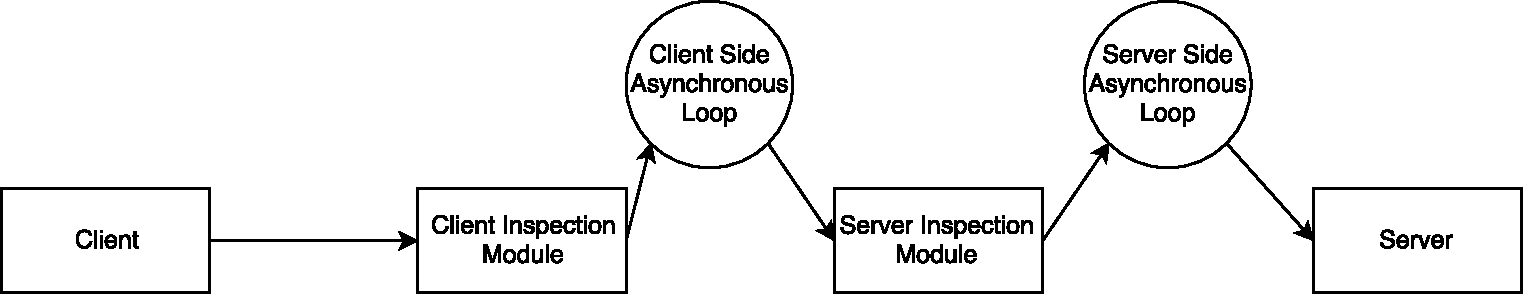
\includegraphics[width=\columnwidth]{figure/async-flow.pdf}
  \vspace{-2mm}
  \caption{The general-purpose asynchronous flow abstraction used in NetStar.}
  \label{fig:async-flow}
  \vspace{-6mm}
\end{figure}

Figure~\ref{fig:async-flow} illustrates our general purpose asynchronous flow abstraction used in NetStar. It is designed to process and inspect connection-oriented flows. It consists of four pluggable part. The client side inspection module aims to mimics the client protocol state. The client side asynchronous loop executes various asynchronous operations. The server side inspection module mimics the server side protocol state while the server side asynchronous loop executes various asynchronous operations as well. The server side asynchronous loop is capable of reconstructing the protocol payload (TCP payload) and analyzing the TCP pay load.

The four parts are pluggable. Programmer can disable uninterested part, making it fully modular. It is designed by combining the Seastar server side programming interface with mOS TCP/IP monitoring sock. 
